\chapter{Resultados y Discusión}

\section{Base de datos implementada}

\par A continuación, se exponen un resumen las propiedades de la base de datos confeccionada, lo cual se muestra en la Tabla \ref{tab:4.1-prop_dataset}.

\begin{table}[H]
    \centering
    \caption{Resumen de las propiedades y distribución del conjunto de datos.}
    \begin{tabular}{|l|c|c|}
        \hline
        \textbf{Subconjunto} & \textbf{Total Imágenes} & \textbf{Total Etiquetas} \\
        \hline
        Entrenamiento (Train) & 1621 & 3755 \\
        \hline
        Validación (Valid) & 461 & 1124 \\
        \hline
        Prueba (Test) & 230 & 491 \\
        \hline
        \textbf{Total} & \textbf{2312} & \textbf{5370} \\
        \hline
    \end{tabular}
    \label{tab:4.1-prop_dataset}
\end{table}

\par A partir del análisis cuantitativo de la base de datos, se generaron dos representaciones gráficas para caracterizar su composición estructural. La Figura \ref{fig:4.1-dataset_classes} ilustra la distribución de frecuencia de las distintas clases de fallas, evidenciando un desbalance entre categorías predominantes y minoritarias. Este comportamiento responde principalmente a la disponibilidad de registros en las fuentes originales. Cabe destacar que se optó por no aplicar técnicas de submuestreo para forzar un balance artificial, dado que, ante la presencia de cruce multiclase (múltiples tipos de fallas coexistiendo en una misma imagen), la eliminación de muestras para equilibrar una categoría habría implicado una pérdida involuntaria de información valiosa para otras clases, priorizándose así la integridad y volumen total del conjunto de datos. \\

\par Por su parte, la Figura \ref{fig:4.1-dataset_split_compo} detalla la organización de las particiones del conjunto de datos (Entrenamiento, Validación y Prueba), distinguiendo la proporción de imágenes que contienen anotaciones respecto a las imágenes de fondo (\textit{background}) utilizadas como control negativo.

\begin{figure}[H]
    \centering
    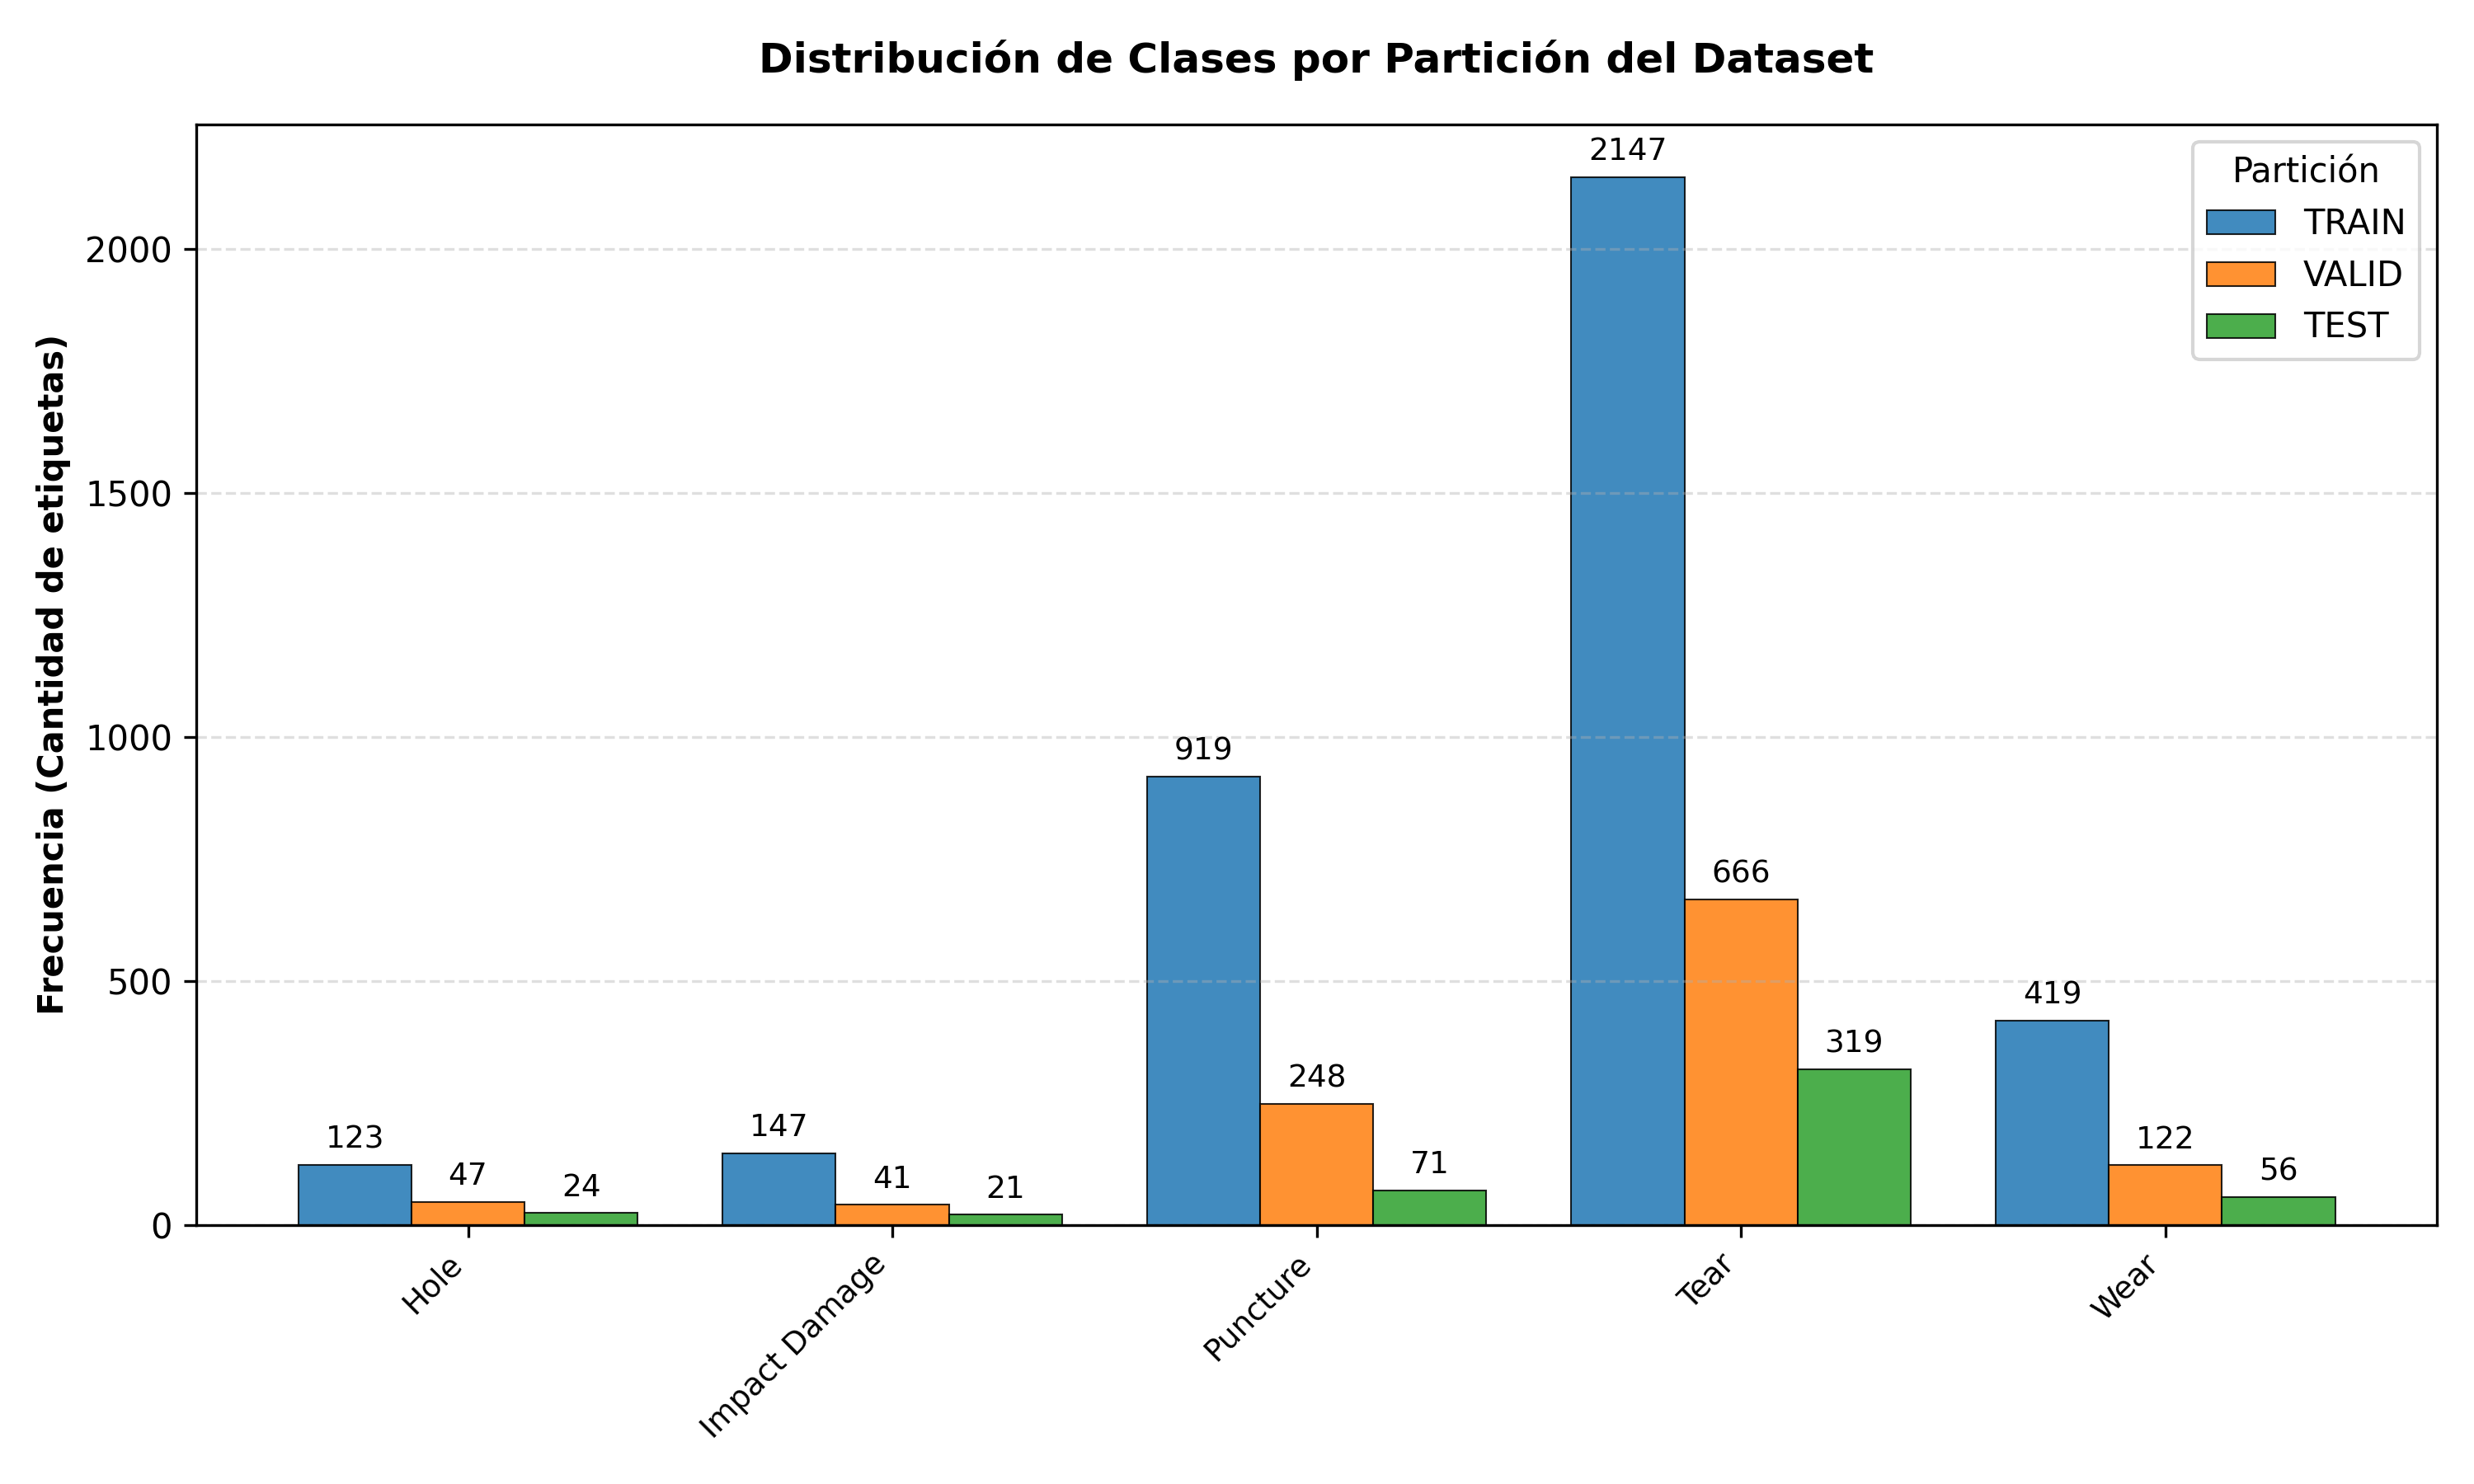
\includegraphics[width=0.8\textwidth]{img/4-Resultados_Discusion/Dataset/class_distribution.png}
    \caption{Distribución de frecuencia de las clases de fallas a través de las particiones del conjunto de datos.}
    \label{fig:4.1-dataset_classes}
\end{figure}

\begin{figure}[H]
    \centering
    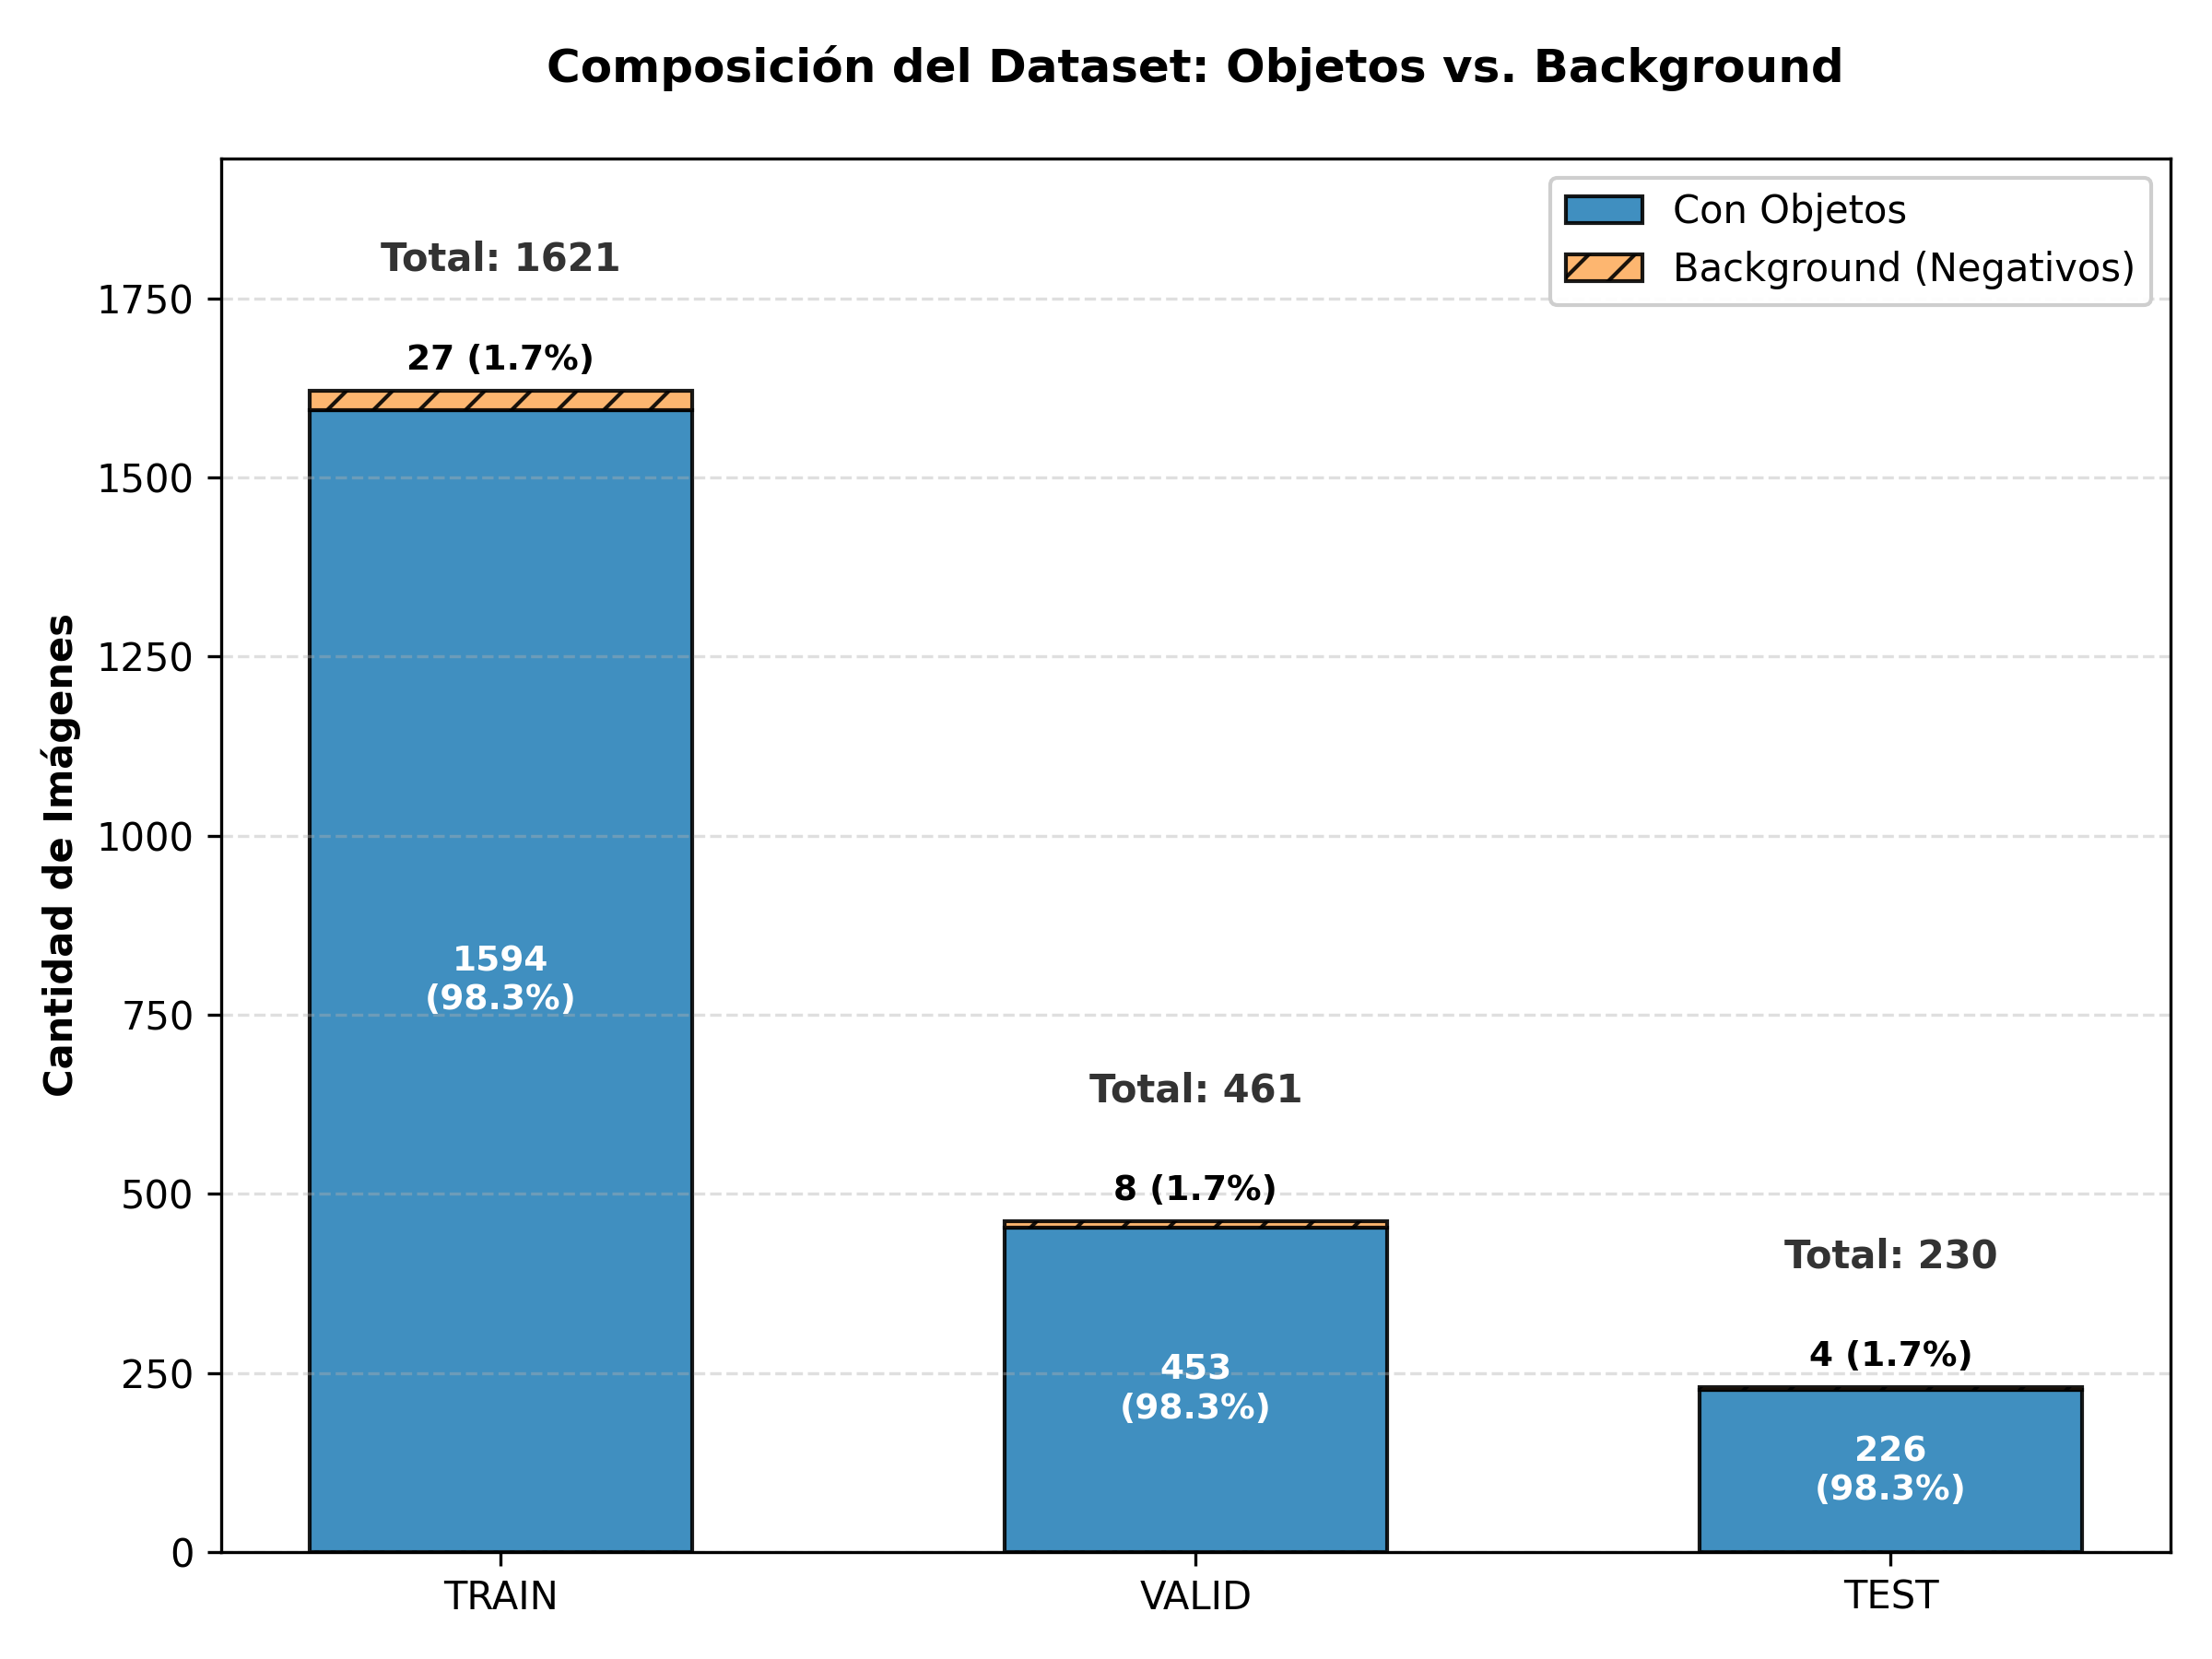
\includegraphics[width=0.8\textwidth]{img/4-Resultados_Discusion/Dataset/split_composition.png}
    \caption{Composición detallada de las particiones del conjunto de datos, diferenciando entre imágenes con objetos y casos de fondo.}
    \label{fig:4.1-dataset_split_compo}
\end{figure}




%%%%%%%%%%%%%%%%%%%%%%%%%%%%%%%%%%%%%%%%%%%%%%%%%%%%%%%%%%%%%%%%%%%%%%%%%%%%%%%%%%%%%%%%%%%%%%%%%%%%%%%%%%%%%%%%%%%%%%%%%%%%%%%%%%%%%%%%%%%%%%%%%%%%%%%%%%%%%%%%%%%%%%%%%%%%%%%%%%%%%%%%%%%%%%%%%%%%%%%%%%%%%%%%%%%%%%%%%%%%%%%%%%%%%%%%%%%%%%%%%%%%%%%%%%%%%%%%%%%%%%%%%%%%%%%%%%%%%%%%%%%%%%%%%%%%%%

\clearpage
\section{Métricas modelos de una sola etapa}


%%%%%%%%%%%%%%%%%%%%%%%%%%%%%%%%%%%%%%%%%%%%%%%%%%%%%%%%%%%%%%%%%%%%%%%%%%%%%%%%%%%%%%%%%%%%%%%%%%
\subsection{YOLOv5}

\par En esta subsección, se exponen y discuten los resultados obtenidos tras el entrenamiento del modelo \textbf{YOLOv5} en su variante \textbf{s} (small), utilizando la configuración de hiperparámetros detallada previamente en la Tabla \ref{tab:3.3-hiperparametros-yolov5}.

% Si alcanzamos, variante x (más pesada), para ver extremos entre velocidad-precision.

%%%%%%%%%%%%%%%%%%%%%%%%%%%%%%%%%%%%%%%%%%%%%%%%%%%%%
\subsubsection{Curva de pérdida vs época por componentes}


%%%%%%%%%%%%%%%%%%%%%%%%%%%%%%%%%%%%%%%%%%%%%%%%%%
\subsubsection{Curva de pérdida vs época promedio}

%%%%%%%%%%%%%%%%%%%%%%%%%%%%%%%%%%%%%%%%%%%%%%%%%%
\subsubsection{Precision y Recall}


%%%%%%%%%%%%%%%%%%%%%%%%%%%%%%%%%%%%%%%%%%%%%%%%%%
\subsubsection{F1-Score}

%%%%%%%%%%%%%%%%%%%%%%%%%%%%%%%%%%%%%%%%%%%%%%%%%%
\subsubsection{Precisión Promedio Media (mAP)}


%%%%%%%%%%%%%%%%%%%%%%%%%%%%%%%%%%%%%%%%%%%%%%%%%%
\subsubsection{Distribución de IoU}

%%%%%%%%%%%%%%%%%%%%%%%%%%%%%%%%%%%%%%%%%%%%%%%%%%
\subsubsection{Matriz de Confusión}



\clearpage
%%%%%%%%%%%%%%%%%%%%%%%%%%%%%%%%%%%%%%%%%%%%%%%%%%%%%%%%%%%%%%%%%%%%%%%%%%%%%%%%%%%%%%%%%%%%%%%%%%%%%%%%%%%%%%%%%%%%%%%%%%%%%%%%%%%%%%%%%%%%%%%%%%%%%%%%%%%%%%%%%%%%%%%%%%%%%%%%%%%%%%%%%%%%%%%%%%%%%%%%%%%%
\subsection{SSD}

\par A continuación, se presentan los resultados obtenidos para el modelo \textbf{SSD300}. Este modelo fue entrenado utilizando una resolución de entrada de $300\times300$ píxeles y la configuración de hiperparámetros detallada en la Tabla \ref{tab:3.4-hiperparametros-ssd}. El análisis se enfoca en evaluar la estabilidad del entrenamiento y la capacidad del detector para operar con mapas de características de menor resolución espacial en comparación con YOLOv5.

%%%%%%%%%%%%%%%%%%%%%%%%%%%%%%%%%%%%%%%%%%%%%%%%%%
\subsubsection{Curva de pérdida vs época específicas}


%%%%%%%%%%%%%%%%%%%%%%%%%%%%%%%%%%%%%%%%%%%%%%%%%%
\subsubsection{Curva de pérdida vs época promedio}

%%%%%%%%%%%%%%%%%%%%%%%%%%%%%%%%%%%%%%%%%%%%%%%%%%
\subsubsection{Precision y Recall}


%%%%%%%%%%%%%%%%%%%%%%%%%%%%%%%%%%%%%%%%%%%%%%%%%%
\subsubsection{F1-Score}


%%%%%%%%%%%%%%%%%%%%%%%%%%%%%%%%%%%%%%%%%%%%%%%%%%
\subsubsection{Precisión Promedio Media (mAP)}



%%%%%%%%%%%%%%%%%%%%%%%%%%%%%%%%%%%%%%%%%%%%%%%%%%
\subsubsection{Distribución de IoU}







%%%%%%%%%%%%%%%%%%%%%%%%%%%%%%%%%%%%%%%%%%%%%%%%%%
\subsubsection{Matriz de Confusión}

\clearpage
